%%
%% This is file `tikzposter-example.tex',
%% generated with the docstrip utility.
%%
%% The original source files were:
%%
%% tikzposter.dtx  (with options: `tikzposter-example.tex')
%%
%% This is a generated file.
%%
%% Copyright (C) 2014 by Pascal Richter, Elena Botoeva, Richard Barnard, and Dirk Surmann
%%
%% This file may be distributed and/or modified under the
%% conditions of the LaTeX Project Public License, either
%% version 2.0 of this license or (at your option) any later
%% version. The latest version of this license is in:
%%
%% http://www.latex-project.org/lppl.txt
%%
%% and version 2.0 or later is part of all distributions of
%% LaTeX version 2013/12/01 or later.
%%

 \documentclass[25pt, a0paper, portrait, margin=0mm, innermargin=15mm,
     blockverticalspace=15mm, colspace=15mm, subcolspace=8mm]{tikzposter} %Default values for poster format options.


\makeatletter
\def\title#1{\gdef\@title{\scalebox{\TP@titletextscale}{%
\begin{minipage}[t]{\linewidth}
\centering
#1
\par
\vspace{0.5em}
\end{minipage}%
}}}
\makeatother

\usepackage{hyperref}
\usepackage{amsmath}
\usepackage{amssymb}
\usepackage{mathtools}


 \tikzposterlatexaffectionproofon %shows small comment on how the poster was made at bottom of poster

 % Commands
 \newcommand{\bs}{\textbackslash}   % backslash
 \newcommand{\cmd}[1]{{\bf \color{red}#1}}   % highlights command


 % Title, Author, Institute



 \title{ Moving from Circles to Spheres...}

 % -- PREDEFINED THEMES ---------------------- %
 % Choose LAYOUT:  Default, Basic, Rays, Simple, Envelope, Wave, Board, Autumn, Desert,
 \usetheme{Default}
\usecolorstyle[colorPalette=Default]{Default}


\begin{document}
\maketitle

\begin{columns}
  \column{0.3}
      \block{Three Cones}{
We seek to compute the normal of the tangent plane\cite{payne1881,softrobotcalc}.
      Consider the three cones that envelope the three spheres
taken in a pair-wise fashion. Let $\theta_{xy}$ be the half-angle of the
aperture of the cone that envelopes sphere $x$ and sphere $y$.
Observe that this plane is tangent to all three cones.

Compute the apices of the three cones, naming the apex of the cone that
envelopes sphere $X$ and sphere $Y$ $\overrightarrow{XY_{apex}}$. It is interesting
to note that the three apices lie on a line, which is where the normal plane
intersects the $XZ$-plane where the center of all the spheres lie.

Let $I_z$ be the $z$ value of the intersection of this line with $z$-axis.

Let the normal of the plane tangent to the three spheres be generated
by a (negative) rotation $\theta_{AB}$ of the $[0,1,0]$ vector about the $Z$-axis followed by a rotation $\gamma$
about the $X$-axis. But what is $\gamma$?
      }
      \column{0.3}
  \block{Definitions}{
    \begin{align}
  \overrightarrow{AB} &= \overrightarrow{A} - \overrightarrow{B} \\
  \overrightarrow{BC} &= \overrightarrow{B} - \overrightarrow{C} \\
  \overrightarrow{CA} &= \overrightarrow{C} - \overrightarrow{A} \\
  \theta_{ab} &= \arcsin{\frac{r_a - r_b}{r_a + r_b}} \\
  \theta_{bc} &= \arcsin{\frac{r_b - r_c}{r_b + r_c}} \\
  \theta_{ca} &= \arcsin{\frac{r_a - r_c}{r_a + r_c}} \\
  \overrightarrow{AB_{apex}} &= \overrightarrow{A} + \hat{\overrightarrow{AB}} \frac{r_a}{\sin{\theta_{ab}}} \\
  \overrightarrow{BC_{apex}} &= \overrightarrow{B} + \hat{\overrightarrow{BC}} \frac{r_b}{\sin{\theta_{bc}}} \\
  \overrightarrow{CA_{apex}} &= \overrightarrow{C} + \hat{\overrightarrow{CA}} \frac{r_c}{\sin{\theta_{ca}}} \\
  \overrightarrow{U} &= \overrightarrow{AB_{apex}} \\
  \overrightarrow{V} &= \overrightarrow{CA_{apex}} \\
  \overrightarrow{W} &= \overrightarrow{BC_{apex}}
\end{align}
    }

              \column{0.4}
            \block{Diagram}{
       \begin{tikzfigure}[Rotation Math]
         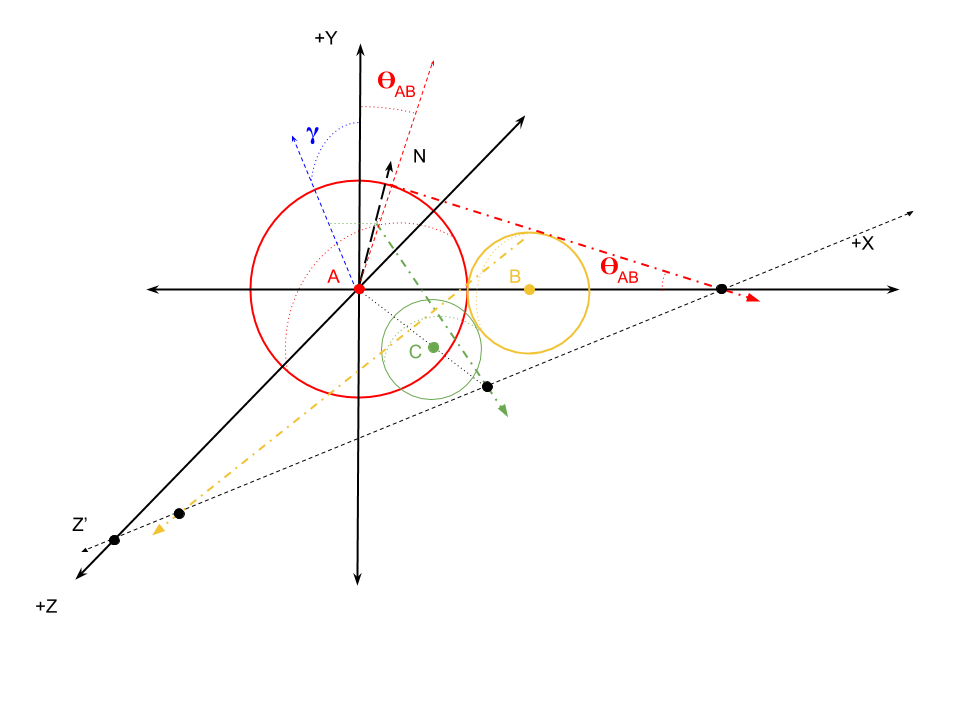
\includegraphics[width=0.325\textwidth]{figures/RotationMath.png}
       \end{tikzfigure}
            }

        \end{columns}
     \begin{columns}
       \column{0.7}

     \block{Three Sphere Math}{


Observe that the $AB$ cone intersects
the $A$ sphere in a circle on the surface of the $A$ perpendicular to and centered on the $X$ axis.

A vector of length $r_A$ that begins pointing in the $X$ direction and is rotated counterclockwise
about the $Z$-axis by $\pi/2 - \alpha$.

However, we must rotate this vector about the $X$ axis by an unknown amount $\theta$ in order
to bring capture the tilt which is not purely a rotation about the $Z$ axis.
Since this angle is computed in the $ZY$ plane, we compute a projection of the point $V$ into
that plane, forming a triangle in the $ZY$ plane.  Call this point $I_z$, the intersection
of the apex line with the $Z$-axis. Let $h$ be the height of the
intersection of the $y$-axis with the $AB$ cone.

\begin{align}
  I_z &= \frac{U_x V_z}{U_x - V_x} \\
  h &= U_x \tan{ \theta_{ab}}  \\
 \gamma &= \arcsin{\frac{h}{I_z}}
\end{align}

Having computed $\theta_{ab}$ and $\gamma$, two rotations give us the plane tanget to all three spheres, and hence in theory the ``tilt'' of our soft Stewart Platform.
     }

        \column{0.2}
         \block{Tentacle}{
         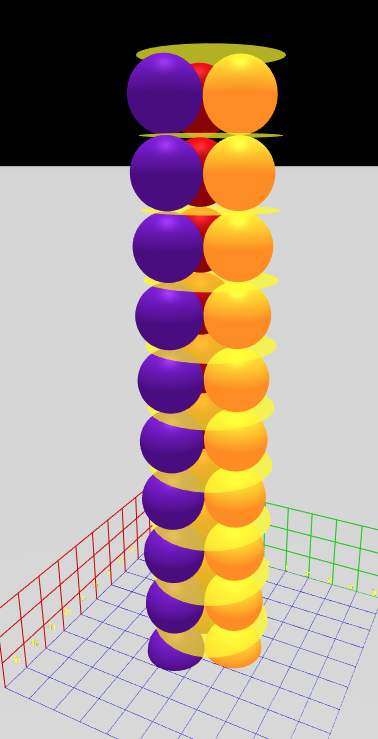
\includegraphics[width=0.15\textwidth]{figures/TentacleConcept.png}
         }
         \end{columns}
\begin{columns}
       \column{0.5}
       \block{Future Work: Inflatable Stewart Platform}{
         By constructing a soft mechanism that serves the same positioning perfomed
         by a mechanical Stewart Platform\cite{wiki:stewart}, we might build
         machines scalable up or down that that are gentle enough to be used
         for medical purposes.

         By solving the problem\cite{payne1881} with
         closed-form expressions as shown here, we allow the possibility of
         computing the derivative of the tilt with respect to change of the radii,
         a function of the pressure in the spheres.
       }
       \column{0.5}
        \block{Future Work: A Soft Tentacle}{
         By stacking such mechanisms, we propose to make a soft {\em tentacle}.
         By composing the derivative of tilt with respect to many such platforms,
         we may construct a Jacobian which allows positioning of the tentacle and
         even motion planning.

         Such a tentacle could be used as an endoscope or arthroscope.
         Because potentially scalable down to minute sizes,
         arterial catheterization may be possible.
       }

     \end{columns}
    \block{Future Work: Joule Heating Phase Change for Inflation}{
            Although inflatable spheres could be controlled by pneumatics,
            it would be more elegant to build a sphere that inflates not
            by air tubes, but with a simple two-wire electrical connection.

           Gas changes pressure when heated, but the change in
            pressure is proportional to the absolute temperature.
            Doubling this temperature is relatively impractical.

            Water or alcohol can be vaporized at
            low temperatures. We hope to design a way to add simple heating wires
            inside an inflatable sphere in order to accomplish a phase change,
            and therefore a drastic pressure change,
            with a simple application of voltage.
          }

  \block{References}{
    \bibliographystyle{acm}
    \bibliography{softrobotmath}
  }



 \end{document}




\endinput
%%
%% End of file `tikzposter-example.tex'.
